\section*{Цель работы}

Целью работы является реализация программы для визуализации графиков
функции распределения случайной величины и функции ее плотности.

Случайная величина удовлетворяет следующим распределениям:
\begin{itemize}
    \item равномерное распределение;
    \item нормальное распределение (номер по списку 10).
\end{itemize}

\section*{Равномерное распределение}

Равномерное распределение задается двумя параметрами: координатами
начала и конца интервала ($a$ и $b$ соответственно). Внутри этого
интервала значение функции плотности принимается постоянным.

Функция плотности распределения:
\begin{equation*}
    а_X(x) = \begin{cases}
        \frac{1}{b - a},\quad\text{если}\quad x \in [a, b]; \\
                0,\quad\text{иначе}.
             \end{cases}
\end{equation*}

Функция распределения:
\begin{equation*}
    F_X(x) = \begin{cases}
                0,\quad x \le a; \\
                \frac{x - a}{b - a},\quad\text{если}\quad x \in (a, b]; \\
                1,\quad\text{иначе}.
             \end{cases}
\end{equation*}

\section*{Нормальное распределение}

Нормальное распределение характеризуется тем, что функция плотности
распределения совпадает с функцией Гаусса. 

Функция плотности распределения:
\begin{equation*}
    f_X(x) = \frac{1}{\sigma \sqrt{2 \pi}} e ^ {-\frac{(x - m)^2}{2 \sigma ^ 2}},
\end{equation*}
где $\mu$ --- математическое ожидание случайной величины, $\sigma$ ---
среднеквадратическое отклонение.

Функция распределения:
\begin{equation*}
    F_X(x) = \frac{1}{\sigma \sqrt{2 \pi}} \int_{-\infty}^{x} e ^ {-\frac{(x - m)^2}{2 \sigma ^ 2}} \mathrm{d}x.
\end{equation*}

\pagebreak

\section*{Результаты работы}

\begin{figure}[h]
    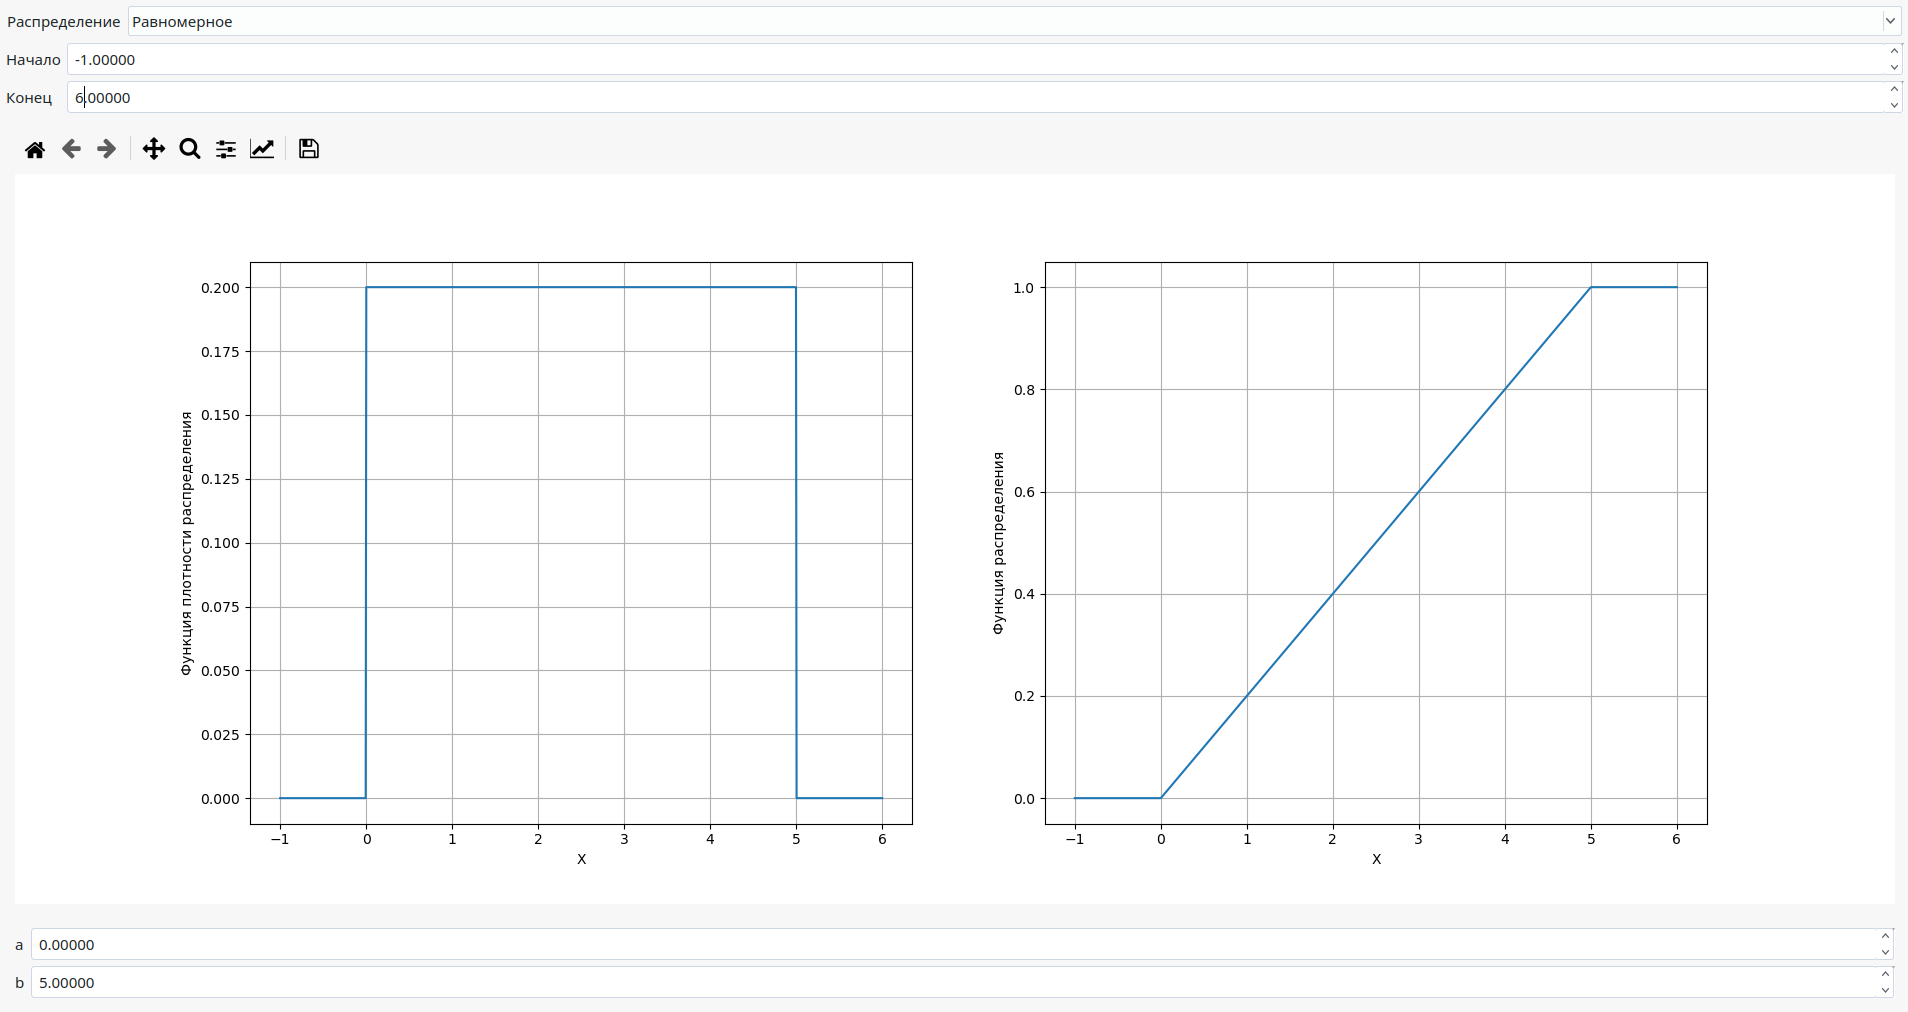
\includegraphics[width=0.9\textwidth]{uniform_general.png}
    \caption{Результаты работы для равномерного распределения с параметрами
             $a=0$, $b=5$}
\end{figure}

\begin{figure}[h]
    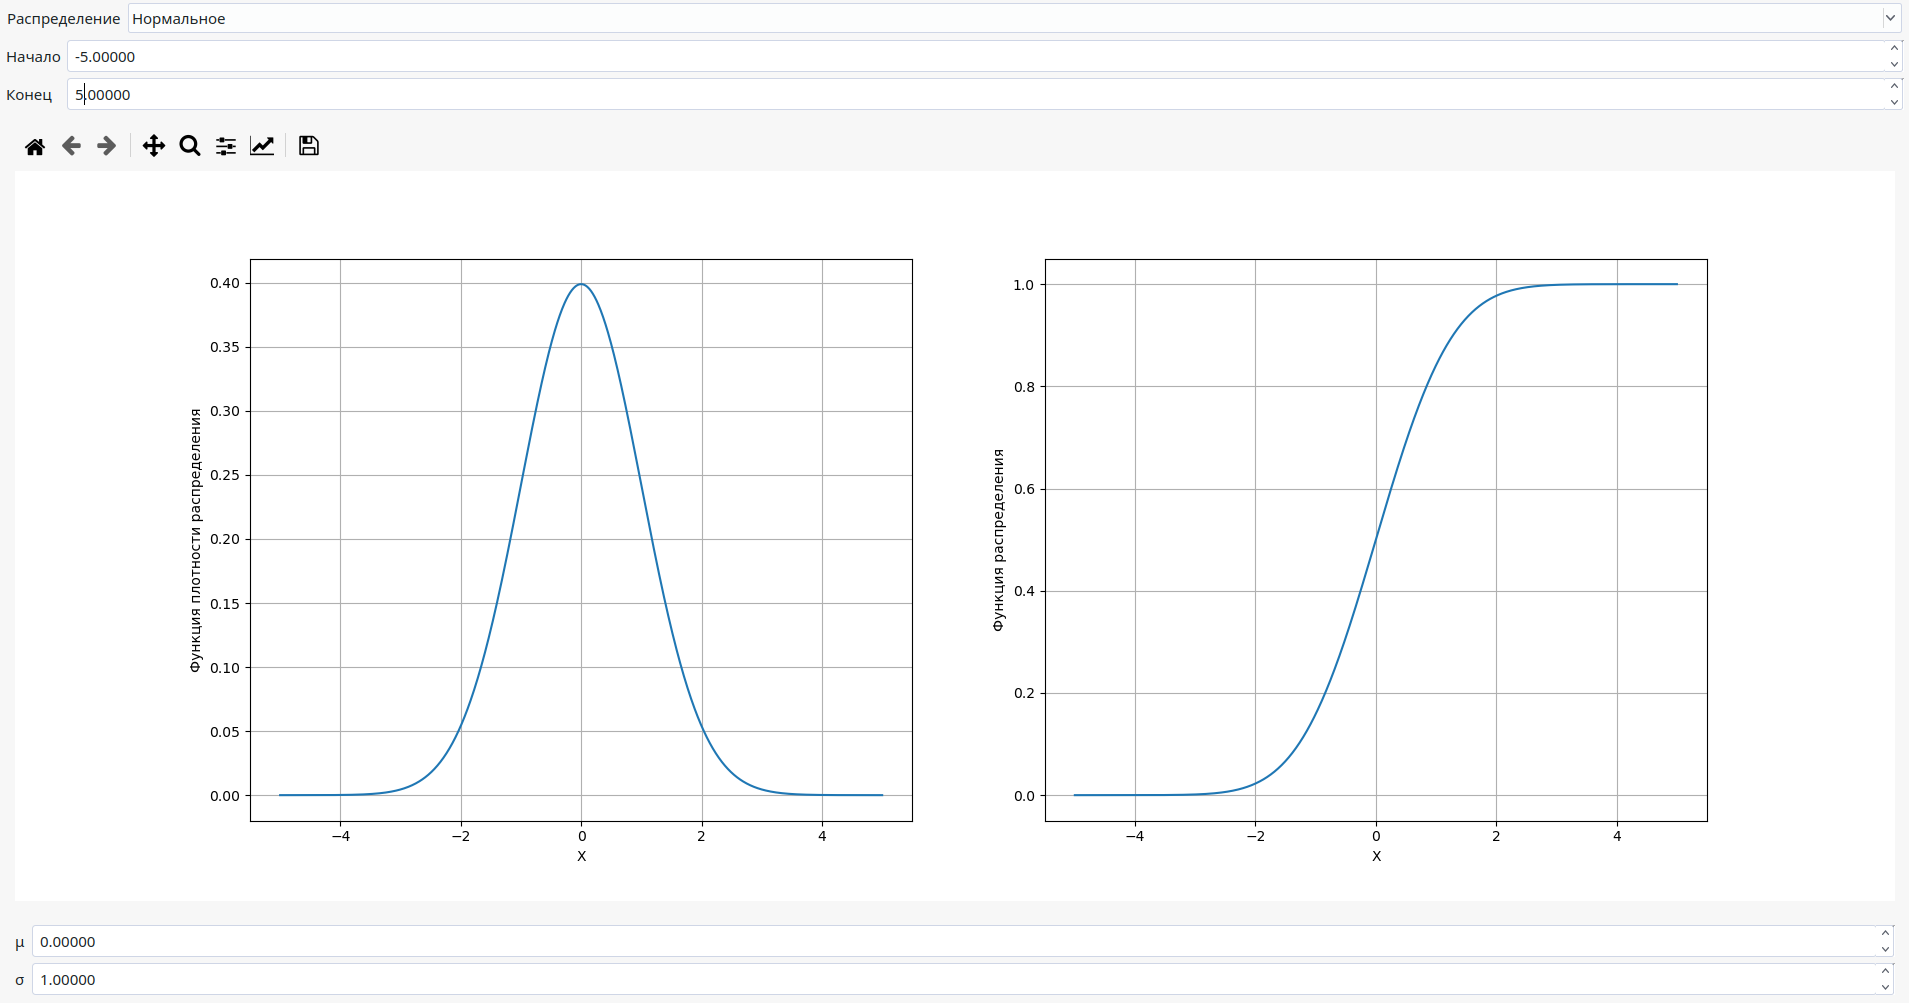
\includegraphics[width=0.9\textwidth]{normal_general.png}
    \caption{Результаты работы для нормального распределения с параметрами
             $\mu=0$, $\sigma=1$}
\end{figure}

\clearpage

\begin{figure}[h]
    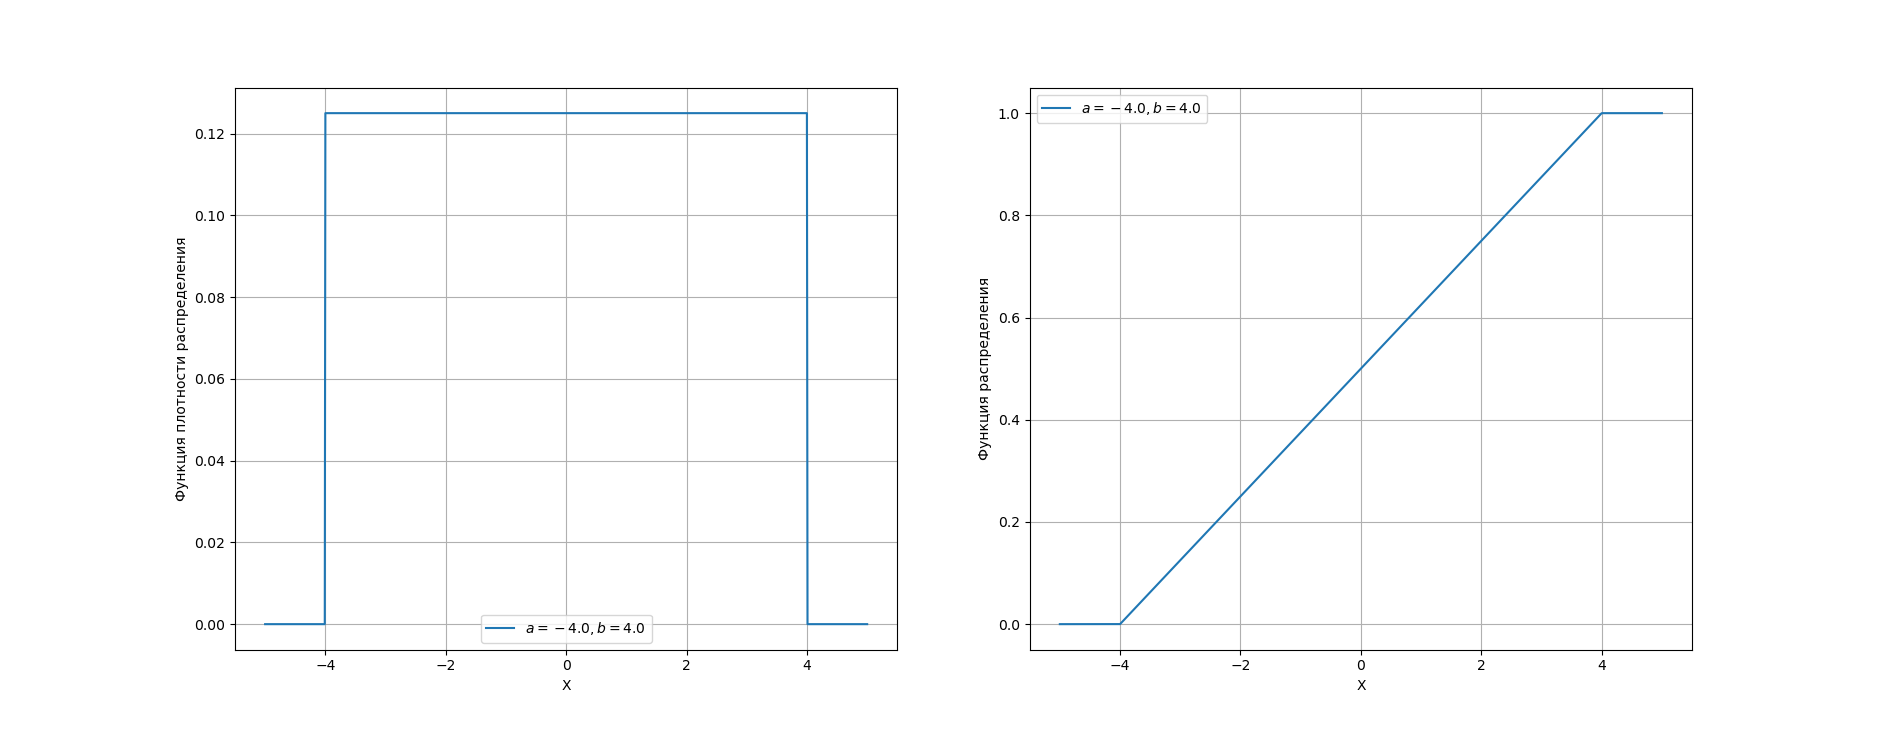
\includegraphics[width=0.9\textwidth]{uniform1.png}
    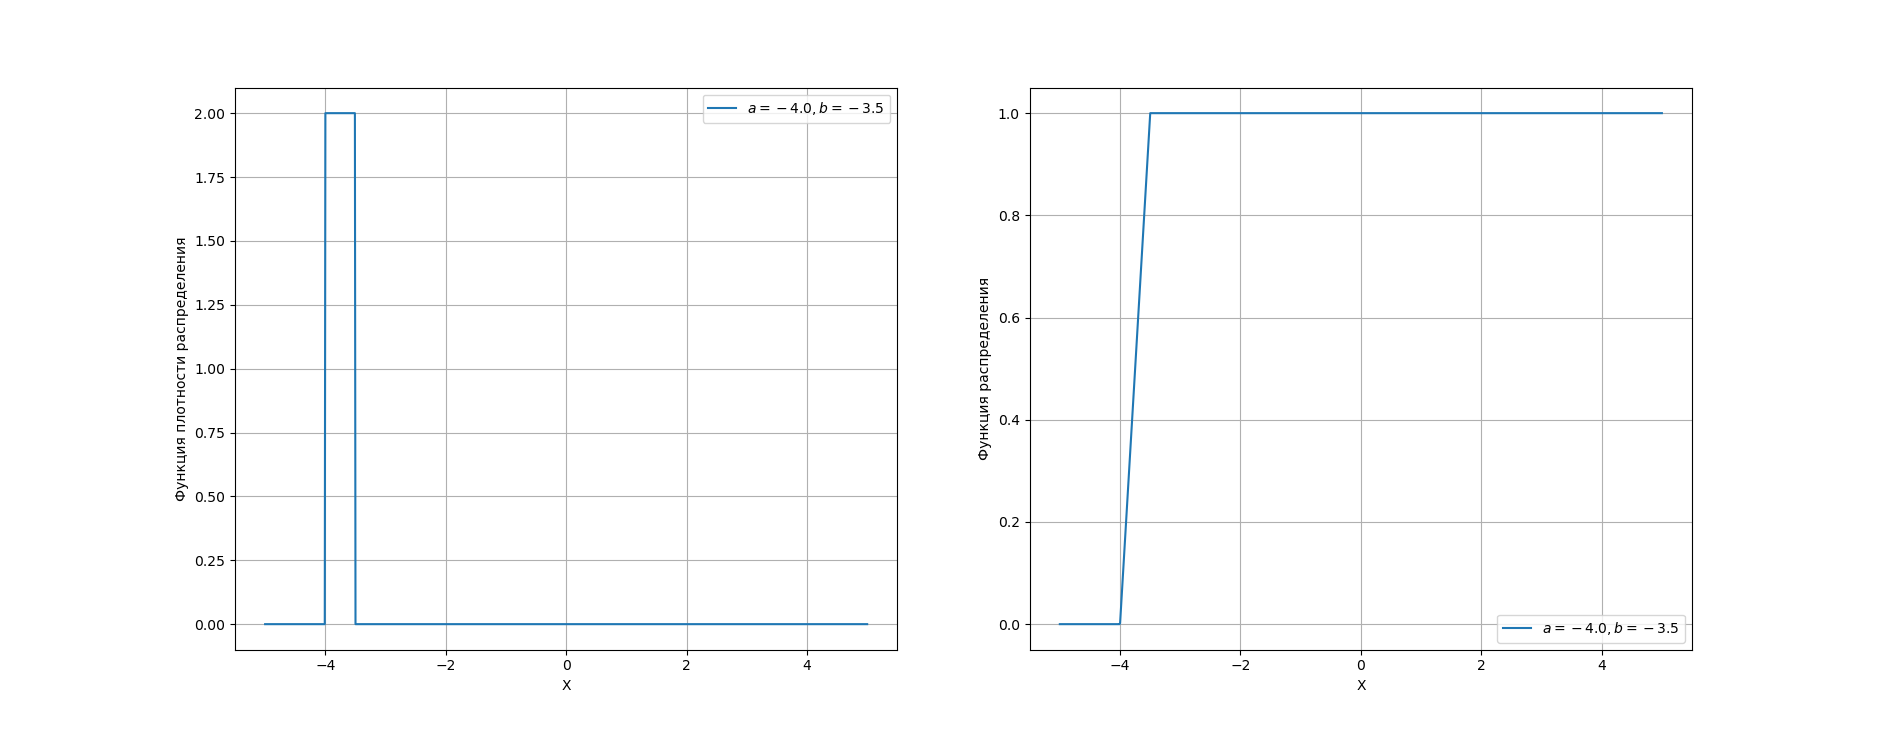
\includegraphics[width=0.9\textwidth]{uniform2.png}
    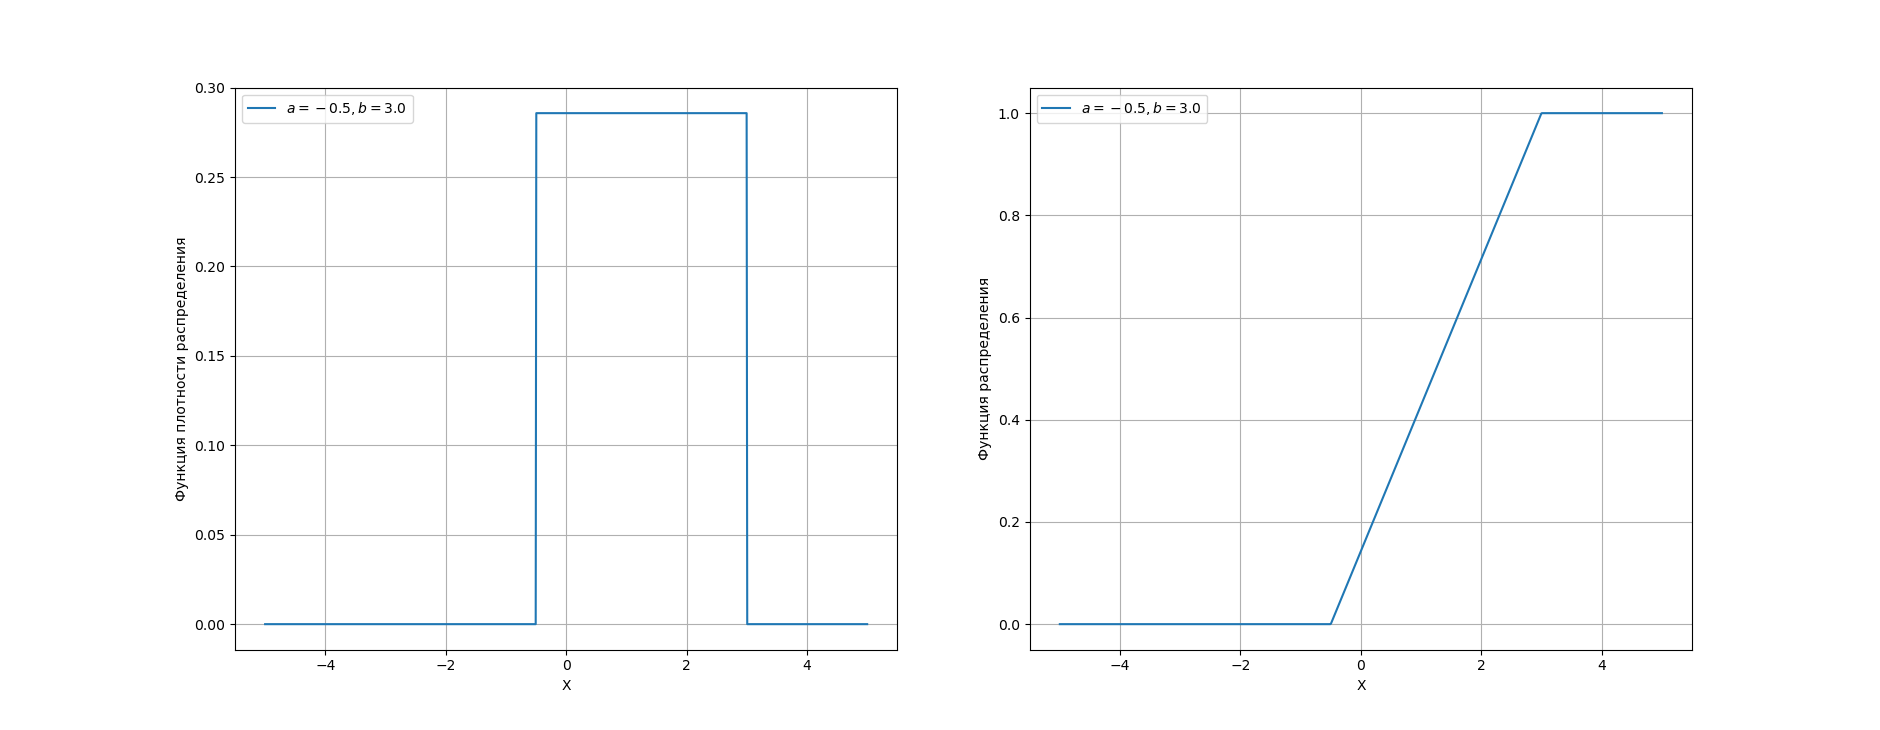
\includegraphics[width=0.9\textwidth]{uniform3.png}
    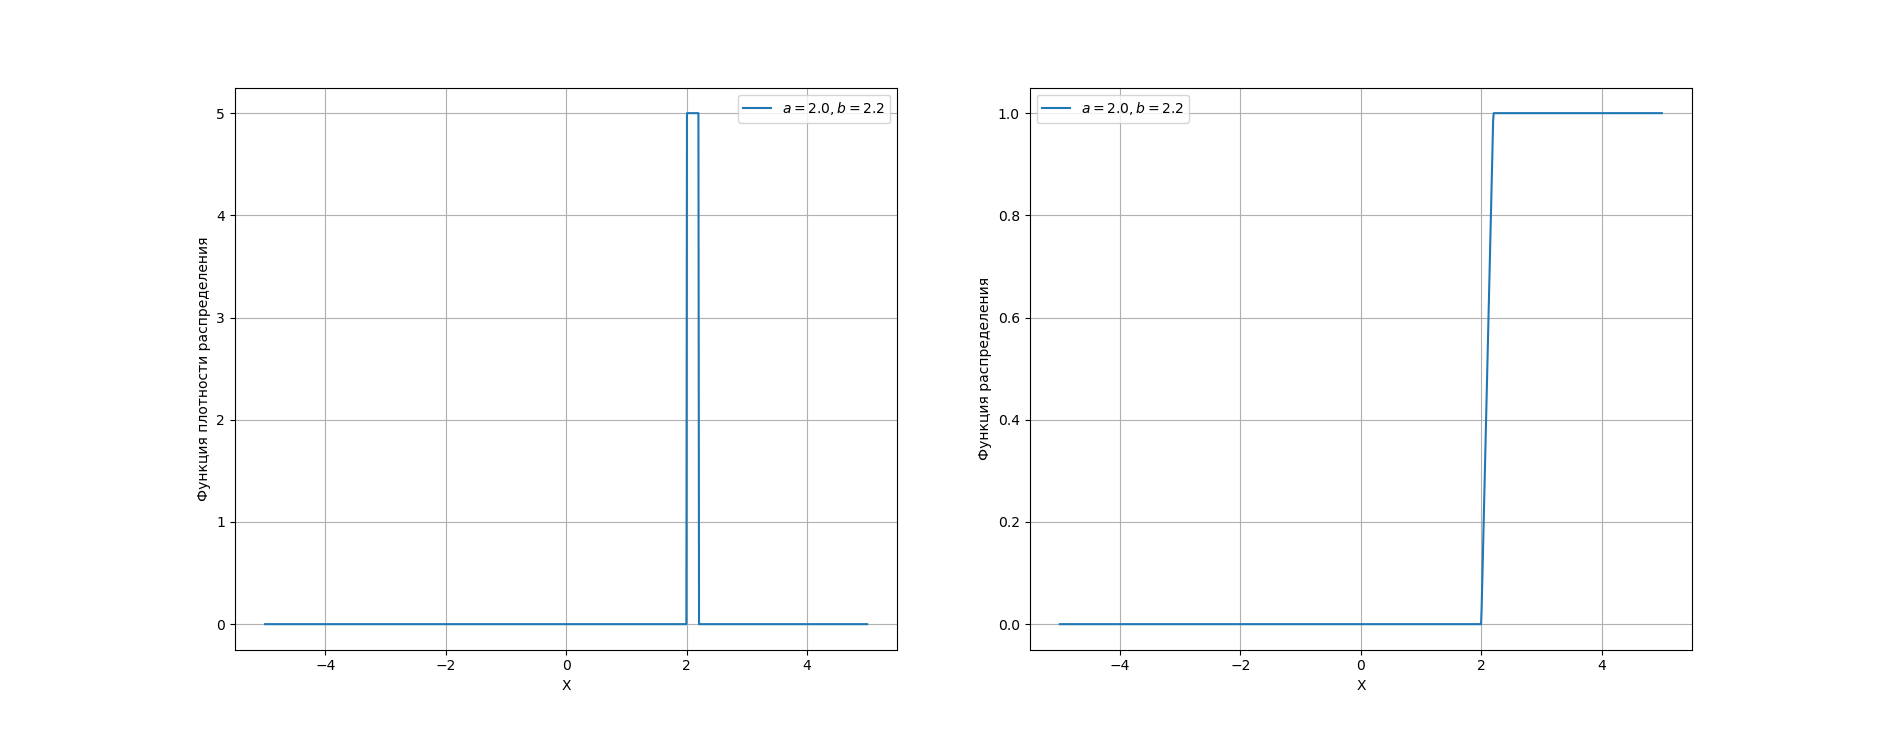
\includegraphics[width=0.9\textwidth]{uniform4.png}
    \caption{Изменение графиков равномерного распределения в зависимости от
             входных параметров}
\end{figure}

\begin{figure}[h]
    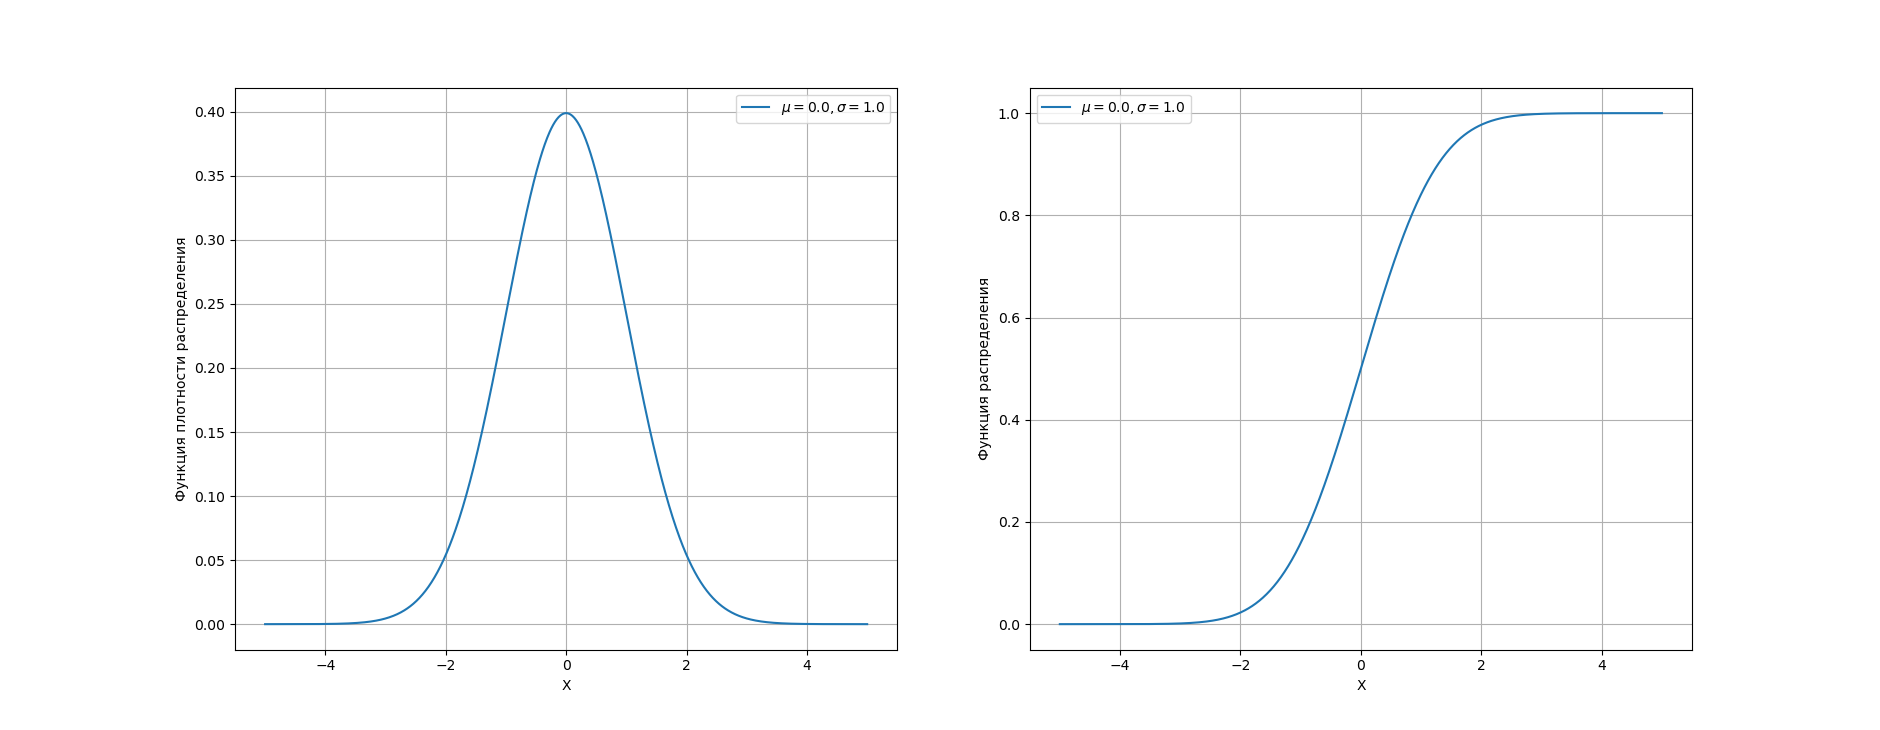
\includegraphics[width=0.9\textwidth]{normal1.png}
    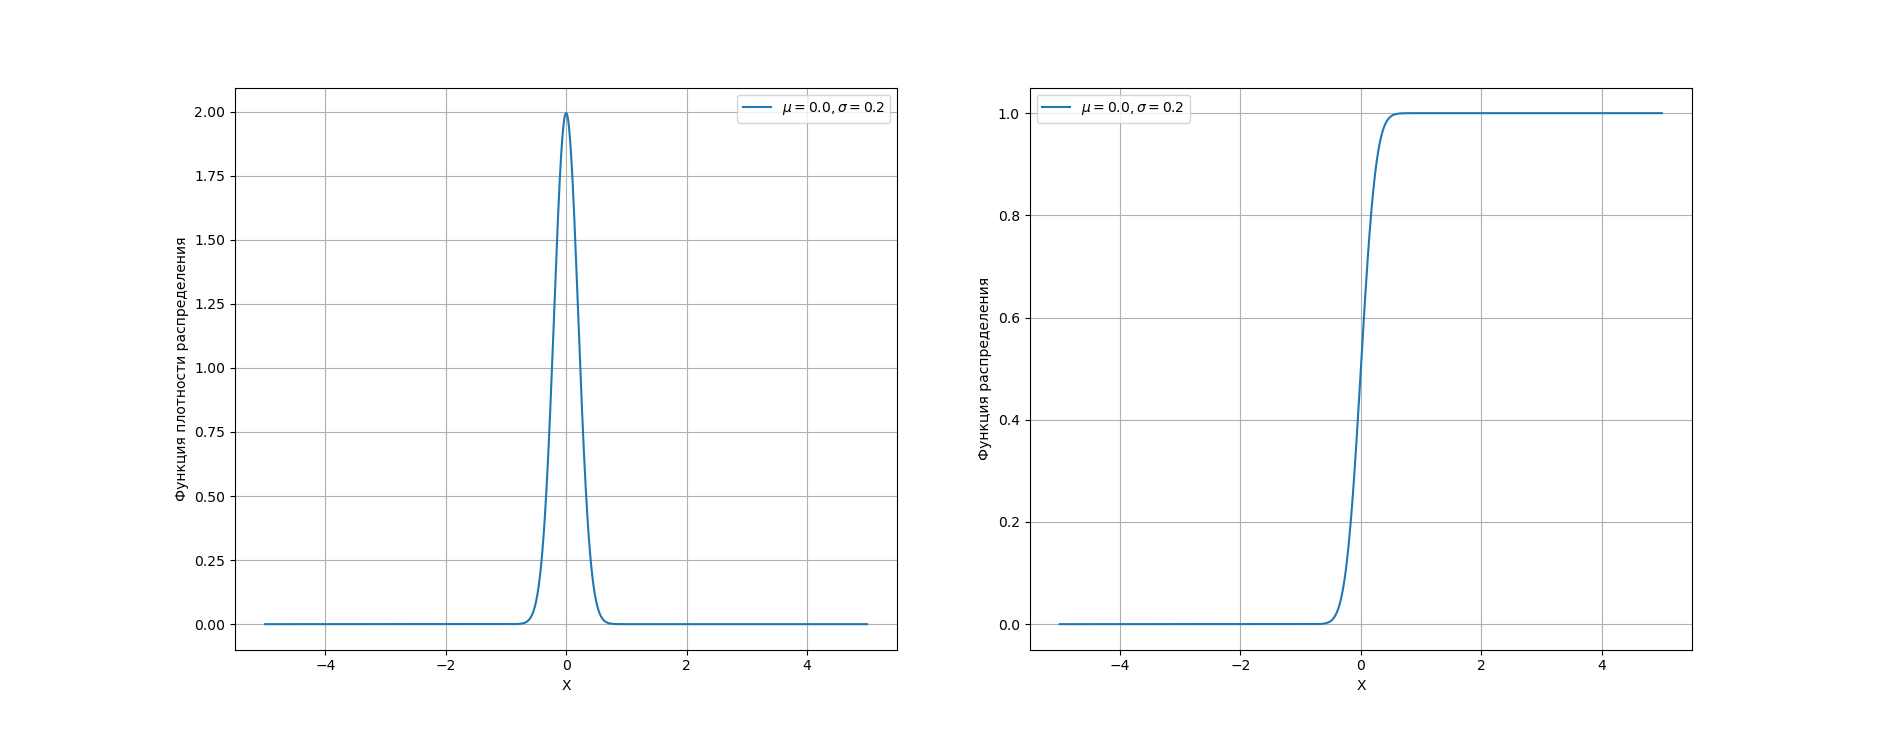
\includegraphics[width=0.9\textwidth]{normal2.png}
    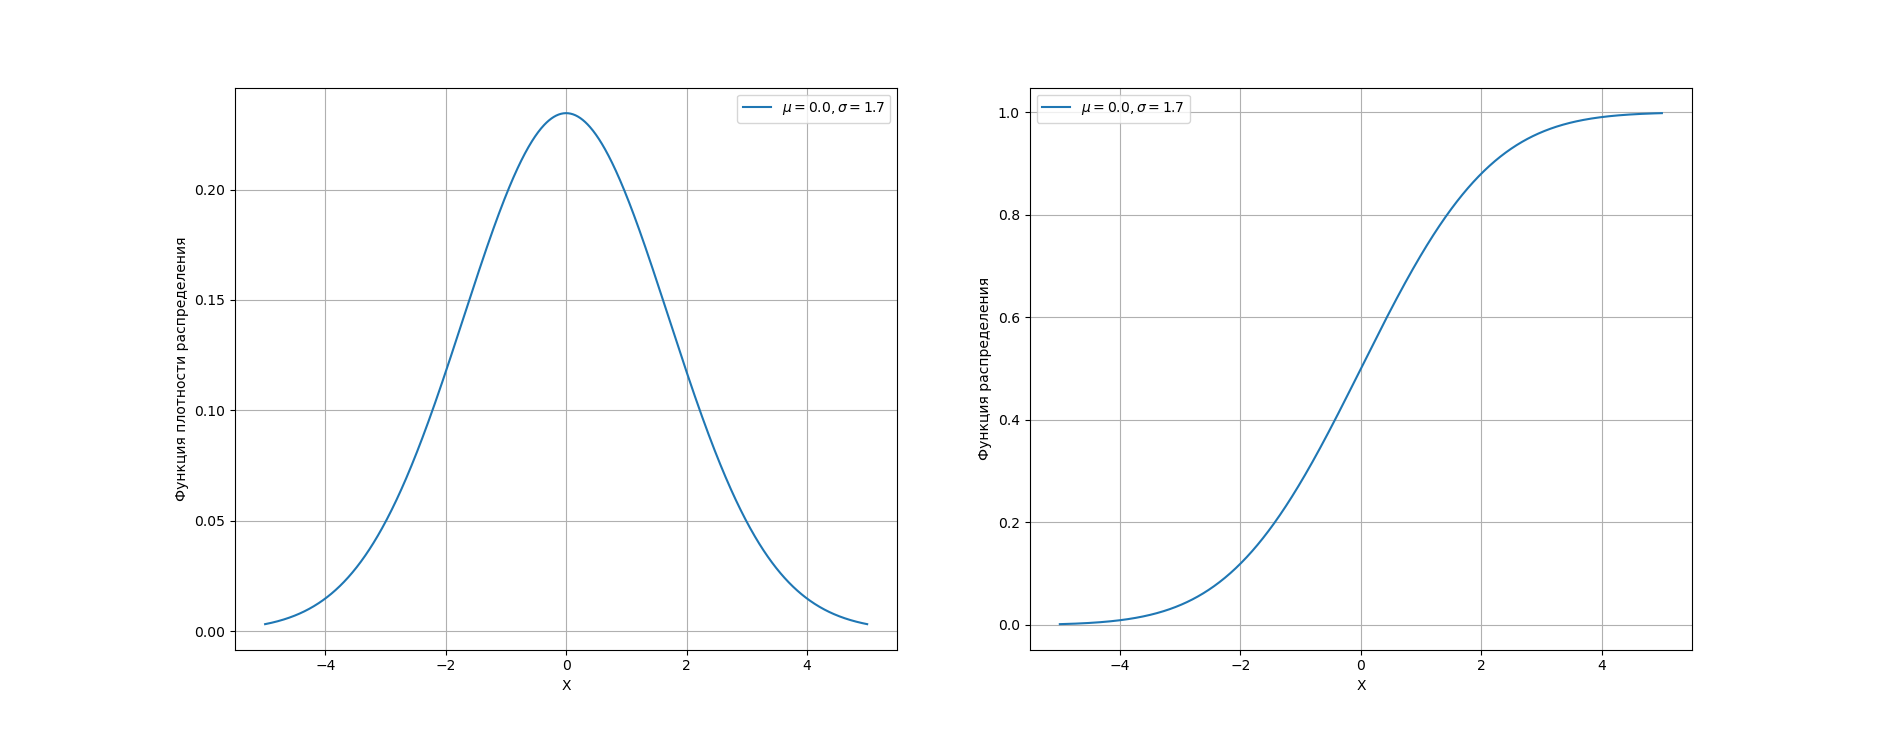
\includegraphics[width=0.9\textwidth]{normal3.png}
    % 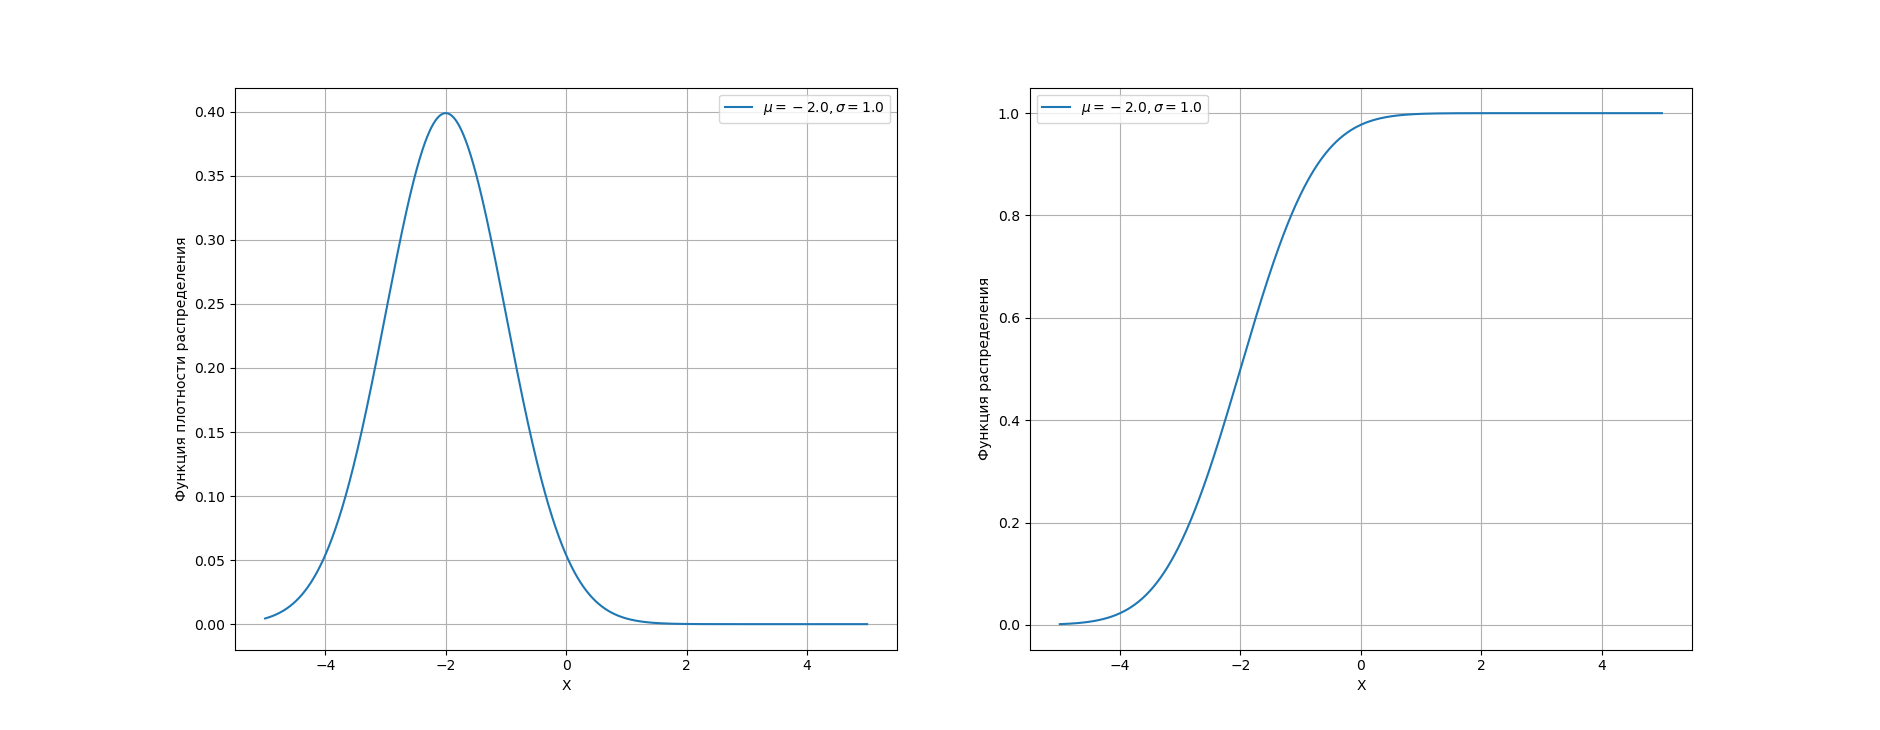
\includegraphics[width=\textwidth]{normal4.png}
    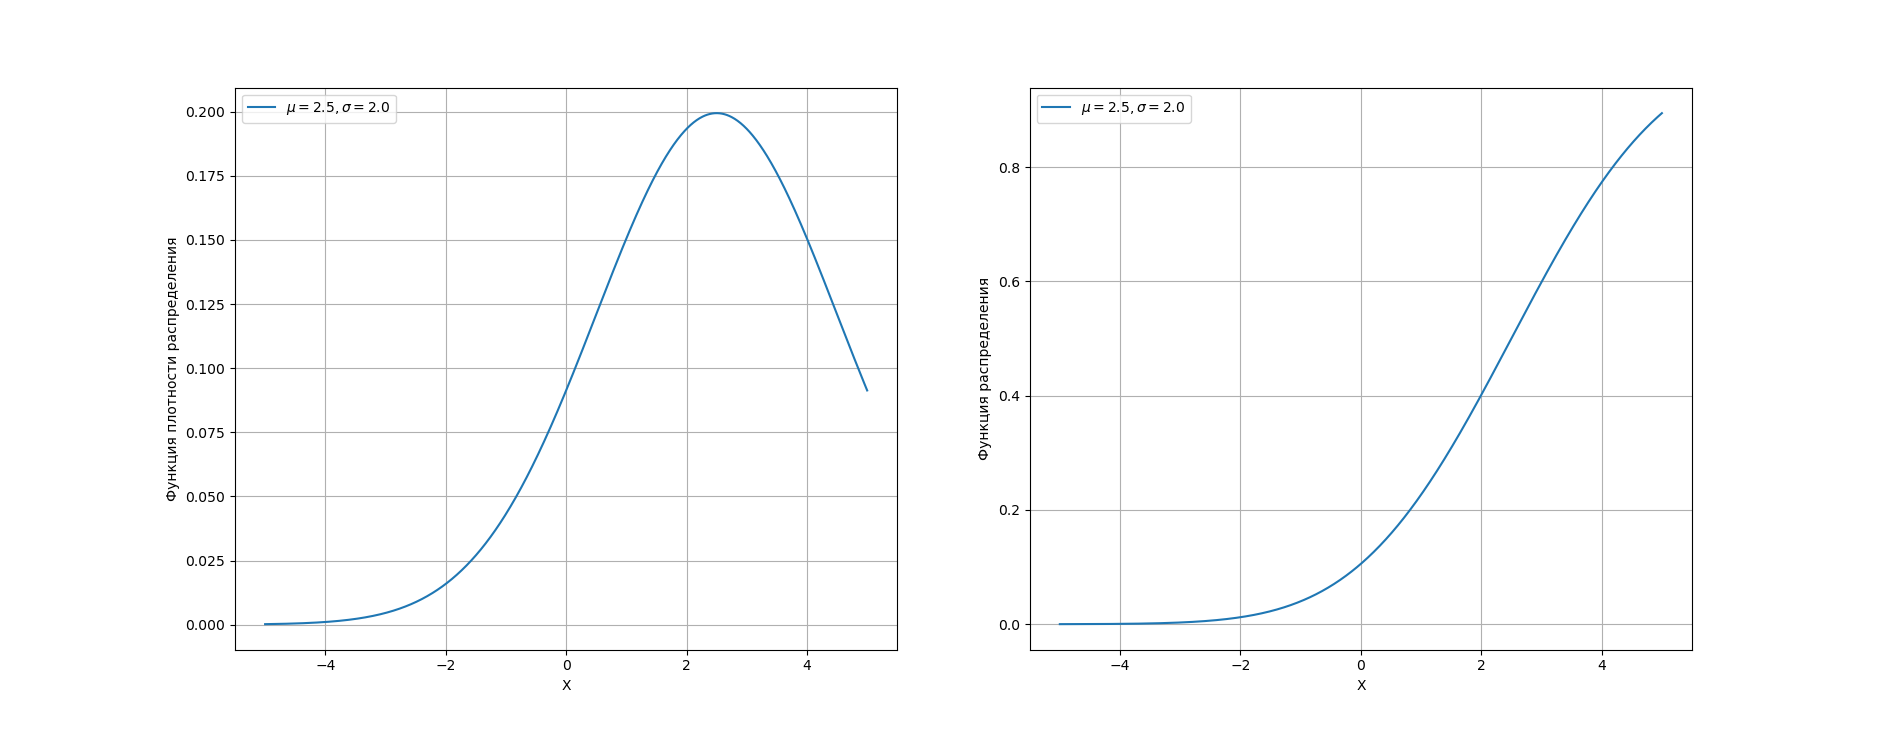
\includegraphics[width=0.9\textwidth]{normal5.png}
    \caption{Изменение графиков нормального распределения в зависимости от
             входных параметров}
\end{figure}

\clearpage

\section*{Вывод}
В ходе выполнения лабораторной работы была разработана программа, позволяющая
строить графики функции распределения и функции плотности распределения
для равномерных и нормальных случайных величин. Были построены и приведены
графики для различных значений входных параметров.

